\section{External Interface Requirements}
\label{sec:external_interface_requirements}%

\subsection{User Interfaces}
\label{subsec:user_interfaces}%
The \verb|CodeKataBattle (CKB)| platform is accessed via an intuitive and responsive web interface compatible with major browsers (Chrome, Firefox, Safari, etc.).
Educators enjoy a dedicated dashboard for effortless creation and management of tournaments, battles, and badges. This dashboard provides a comprehensive view of ongoing battles, tournament scores, and badge achievements.
Students utilize a user-friendly dashboard for team formation, battle participation, and progress tracking. It streamlines team formation, displays upcoming battles, current ranks, and summarizes earned badges.
GitHub seamlessly integrates into the platform for code versioning and automated testing. Students can easily fork repositories, set up GitHub Actions, and monitor build and test results within the \verb|CKB| platform.
To keep all stakeholders informed, the platform employs a robust notification system. This system supports both email notifications and in-platform alerts, 
ensuring timely updates for educators and students on critical events like upcoming deadlines or changes in battle status.

\subsection{Hardware Interfaces}
\label{subsec:hardware_interfaces}%
The \verb|CKB| platform prioritizes accessibility by ensuring compatibility across a diverse range of devices. 
Users can seamlessly access the platform from desktop computers, laptops, tablets, and smartphones. This inclusivity caters to the varied preferences and device usage patterns of our user base. 
The platform's responsive design ensures that the user interface adapts fluidly to different screen sizes, providing an optimal experience regardless of the device used. 
This commitment to device compatibility aims to enhance user convenience and flexibility, promoting a versatile and user-centric engagement with the \verb|CKB| platform.

\subsection{Software Interfaces}
\label{subsec:software_interfaces}%
The \verb|CKB| platform seamlessly communicates with GitHub via APIs, enabling functionalities such as repository creation, commit tracking, and automated test processes.
To ensure a secure integration, the platform should smoothly connect with GitHub APIs, facilitating automated workflows triggered by student commits.
Additionally, the platform harnesses static analysis tools to assess code quality comprehensively.
Incorporating these tools seamlessly, educators can tailor automated evaluations by configuring specific aspects like security, reliability, and maintainability. This flexibility ensures a nuanced understanding of the code's overall quality.

\subsection{Communication Interfaces}
\label{subsec:communication_interfaces}%
The platform actively engages in communication with students, delivering notifications, battle updates, and final results in a secure manner through HTTPS. A reliable messaging system ensures timely information dissemination to students.
Similarly, educators stay well-informed through the platform, receiving notifications and updates on battle progress and final results. Secure communication channels, similar to those used for students, guarantee the confidentiality and reliability of information relayed to educators.
For the configuration of badges and rules, educators seamlessly use the platform to define new badges, rules, and associated variables. Ensuring a user-friendly interface, educators can make real-time adjustments, with changes promptly reflecting across the platform. This intuitive process empowers educators to tailor the platform to their evolving requirements effortlessly.

\section{Functional Requirements}
\label{sec:functional_requirements}%

\subsection{Requirements}
\label{subsec: requirements}%
The \verb|CKB| platform offers several functionalities to both educators and students.
In the following table they are listed all the detected requirements that the platform should respect in order to guarantee
the satisfiability of the goals:
\newpage
\newcounter{req}
\setcounter{req}{1}
\newcommand{\creq}{\thereq\stepcounter{req}}
\textbf{Educators}
\begin{center}
    \begin{longtable}{|l|p{0.9\linewidth}|}
        \hline
        \textbf{ID} & \textbf{Description}                                                                                                                             \\
        \hline
        R\creq      & The \verb|CKB| platform shall allow educators to create an account.                                                                    \\
        \hline
        R\creq      & The \verb|CKB| platform shall allow educators to log in.                                                                                 \\
        \hline
        R\creq      & The \verb|CKB| platform shall allow educators to create a new tournament.                                                                \\
        \hline
        R\creq      & The \verb|CKB| platform shall allow educators to set the minimum and maximum number of students per group for a tournament.                                                        \\
        \hline
        R\creq      & The \verb|CKB| platform shall allow educators to upload a code kata battle.                                                                         \\
        \hline
        R\creq      & The \verb|CKB| platform shall allow educators to grant permissions to other educators to create battles within a specific tournament.                                                      \\
        \hline
        R\creq      & The \verb|CKB| platform shall enable educators to include a battle to a specific tournament.                                                      \\
        \hline
        R\creq      & The \verb|CKB| platform shall allow educators to include a description for a battle.                                                                \\
        \hline
        R\creq      & The \verb|CKB| platform shall allow educators to include a software project with test cases.                                                                \\
        \hline
        R\creq      & The \verb|CKB| platform shall allow educators to set a registration deadline for a battle within a tournament.                                          \\
        \hline
        R\creq      & The \verb|CKB| platform shall allow educators to set a final submission deadline for a battle within a tournament.                                                                  \\
        \hline
        R\creq      & The \verb|CKB| platform shall allow educators to set additional configurations for scoring, including functional aspects and quality level criteria.                               \\
        \hline
        R\creq      & The \verb|CKB| platform shall allow educators to close a tournament.                                                  \\
        \hline
        R\creq      & The \verb|CKB| platform shall allow an educator to define optional manual evaluation criteria for score assignment in battles.   \\
        \hline
        R\creq      & The \verb|CKB| platform shall allow educators to manually evaluate and assign scores to teams.                                           \\
        \hline
        R\creq      & The \verb|CKB| platform shall allow educators and students to visualize the gamification badges.                                                      \\
        \hline
        R\creq      & The \verb|CKB| platform shall allow educators to define new badges for gamification.                                                             \\
        \hline
        R\creq      & The \verb|CKB| platform shall allow educators to define new rules associated with the badges.                                                      \\
        \hline
        R\creq      & The \verb|CKB| platform shall allow educators to define new variables associated with the badges.                                                      \\
        \hline
        R\creq      & The \verb|CKB| platform shall allow all students and educators to see the ranking of each ongoing tournament with the score of each student subscribed.\\
        \hline
        \caption{Educator Requirements.}
        \label{tab: req}%
    \end{longtable}
\end{center}

\textbf{Students}
\begin{center}
    \begin{longtable}{|l|p{0.9\linewidth}|}
        \hline
        \textbf{ID} & \textbf{Description}                                                                                                                             \\
        \hline
        R\creq      & The \verb|CKB| platform shall not allow students to participate a tournament after the registration deadline.                                                      \\
        \hline
        R\creq      & The \verb|CKB| platform shall not allow students to participate a battle after the registration deadline.                                                      \\
        \hline
        R\creq      & The \verb|CKB| platform shall allow students to subscribe to a tournament within a specified deadline.                                                  \\
        \hline
        R\creq      & The \verb|CKB| platform shall allow students to create teams for a specific battle within a tournament.                                                      \\
        \hline
        R\creq      & The \verb|CKB| platform shall allow students to join teams for a specific battle within a tournament.                                                      \\
        \hline
        R\creq      & The \verb|CKB| platform shall allow students to invite other participants to the same group.                               \\
        \hline
        R\creq      & The \verb|CKB| platform shall allow students to accept an invitation.                               \\
        \hline
        R\creq      & The \verb|CKB| platform shall allow students to reject an invitation.                               \\
        \hline
        R\creq      & The \verb|CKB| platform shall allow students to join a battle without a team.                               \\
        \hline
        R\creq      & The \verb|CKB| platform shall allow students to upload a solution for a specific battle on behalf of the team.                                                      \\
        \hline
        \caption{Student Requirements.}
        \label{tab: req}%
    \end{longtable}
\end{center}

\textbf{Platform}
\begin{center}
    \begin{longtable}{|l|p{0.9\linewidth}|}
        \hline
        \textbf{ID} & \textbf{Description}                                                                                                                             \\
        \hline
        R\creq      & The \verb|CKB| platform shall notify all subscribed students of a new battle and its details within a specific tournament.                               \\
        \hline
        R\creq      & The \verb|CKB| platform shall notify all subscribed students of a new tournament and its details.                               \\
        \hline
        R\creq      & The \verb|CKB| platform shall create a GitHub repository for each battle.                                        \\
        \hline
        R\creq      & send a link to the Github repository associated to a battle to all members of subscribed teams upon expiration of the registration deadline. \\
        \hline
        R\creq      & The \verb|CKB| platform shall be able to be informed of new students' commits by Github Actions workflows. \\
        \hline
        R\creq      & The \verb|CKB| platform shall be able to pull the latest sources from the forks of the Github repository provided. \\
        \hline
        R\creq      & The \verb|CKB| platform shall be able to run the testcases on the code uploaded by students and determine if the code is a valid solution for the exercise.\\
        \hline
        R\creq      & The \verb|CKB| platform shall inform students of the mandatory automated evaluation criteria, including functional aspects, timeliness, and source code quality.                                        \\
        \hline
        R\creq      & The \verb|CKB| platform shall automatically update the battle score of a team based on GitHub commits and test results.                                   \\
        \hline
        R\creq      & The \verb|CKB| platform shall automatically close a finished battle.                                                      \\
        \hline
        R\creq      & The \verb|CKB| platform shall assign or update battle scores to each team of the battle.                                                      \\
        \hline
        R\creq      & The \verb|CKB| platform shall calculate and update the personal tournament score of each student based on their performance in battles.                    \\
        \hline
        R\creq      & The \verb|CKB| platform shall be able to create a ranking of teams for every tournament.                                                      \\
        \hline
        R\creq      & The \verb|CKB| platform shall keep track of time elapsed from the start of a CKB and the final submissions of each team. \\
        \hline
        R\creq      & The \verb|CKB| platform shall be able to use static analysis tools to evaluate the quality of the code submitted by teams in terms of security, reliability, maintainability and other aspects defined by the educator who created the battle. \\
        \hline
        R\creq      & The \verb|CKB| platform shall notify all students involved in a tournament when it is closed and the final ranking is available.                                                       \\
        \hline
        R\creq      & The \verb|CKB| platform shall visualize ongoing tournaments and their ranks for all users.                                                                 \\
        \hline
        R\creq      & The \verb|CKB| platform shall display collected badges on the profile of both students and educators.                                                                    \\
        \hline
        \caption{Platform Requirements.}
        \label{tab: req}%
    \end{longtable}
\end{center}

\subsection{Mapping on goals}
\label{subsec: map_on_g}%
In the following section it is shown how the relation $R\land D \models G$ holds.
In particular, at first it is shown a traceability matrix that associates domain assumptions and requirements to each goal.
After that, to facilitate reading, the section reports the text of all the assumptions and all the requirements related to each goal.
\newcounter{mg}
\setcounter{mg}{1}
\newcommand{\cmg}{\themg\stepcounter{mg}}
\begin{center}
    \begin{longtable}{|p{0.06\linewidth}|p{0.34\linewidth}|p{0.6\linewidth}|}
        \hline
        \textbf{Goal} & \textbf{Domain assumptions}                       & \textbf{Requirements}                                                               \\
        \hline
        G\cmg         &                             & R23, R24, R25, R29, R30                        \\
        \hline
        G\cmg         &                             & R24, R25, R26, R27, R28                                      \\
        \hline
        G\cmg         &                             & R1, R2, R3, R4, R5, R6, R7, R8, R9, R10, R11, R12, R13, R14, R15, R16, R17, R18, R19, R20                                \\
        \hline
        G\cmg         &                             & R33, R34, R35, R36, R37, R38, R39              \\
        \hline
        G\cmg         &                             & R20, R29, R30, R44                               \\
        \hline
        G\cmg         &                             & R41, R42, R45                     \\
        \hline
        G\cmg         &                             & R46, R47                                \\
        \hline
        G\cmg         &                             & R48                                                   \\
        \hline
        G\cmg         &                             & R16, R17, R18, R19, R48                                               \\
        \hline
        \caption{Mapping on goals.}
        \label{tab: map_on_g}%
    \end{longtable}
\end{center}

In this section, it will be shown the functional requirements and the domain assumption related to each goal.
\begin{itemize}

    \item \textbf{{[G.1]} Enable students to enhance their software development skills through coding challenges.}
    \begin{itemize}
        \item \textbf{[R.23]} The \verb|CKB| platform shall allow students to subscribe to a tournament within a specified deadline.
        \item \textbf{[R.24]} The \verb|CKB| platform shall allow students to create teams for a specific battle within a tournament.
        \item \textbf{[R.25]} The \verb|CKB| platform shall allow students to join teams for a specific battle within a tournament. 
        \item \textbf{[R.29]} The \verb|CKB| platform shall allow students to join a battle without a team. 
        \item \textbf{[R.30]} The \verb|CKB| platform shall allow students to upload a solution for a specific battle on behalf of the team.
        \item \textbf{[D.1]}
    \end{itemize}

    \item \textbf{{[G.2]} Facilitate peer learning and collaboration by allowing students to form teams and work together on coding exercises. }
        \begin{itemize}
            \item \textbf{[R.24]} The \verb|CKB| platform shall allow students to create teams for a specific battle within a tournament.
            \item \textbf{[R.25]} The \verb|CKB| platform shall allow students to join teams for a specific battle within a tournament.
            \item \textbf{[R.26]} The \verb|CKB| platform shall allow students to invite other participants to the same group. 
            \item \textbf{[R.27]} The \verb|CKB| platform shall allow students to join a battle without a team.
            \item \textbf{[R.28]} The \verb|CKB| platform shall allow students to reject an invitation.
            \item \textbf{[D.1]}
        \end{itemize}

        \item \textbf{{[G.3]} Provide educators with a platform to create and manage coding challenges tailored to specific learning objectives. }
        \begin{itemize}
            \item \textbf{[R.1]} The \verb|CKB| platform shall allow educators to create an account.
            \item \textbf{[R.2]} The \verb|CKB| platform shall allow educators to log in. 
            \item \textbf{[R.3]} The \verb|CKB| platform shall allow educators to create a new tournament.
            \item \textbf{[R.4]} The \verb|CKB| platform shall allow educators to set the minimum and maximum number of students per group for a tournament.
            \item \textbf{[R.5]} The \verb|CKB| platform shall allow educators to upload a code kata battle.
            \item \textbf{[R.6]} The \verb|CKB| platform shall allow educators to grant permissions to other educators to create battles within a specific tournament.
            \item \textbf{[R.7]} The \verb|CKB| platform shall enable educators to include a battle to a specific tournament. 
            \item \textbf{[R.8]} The \verb|CKB| platform shall allow educators to include a description for a battle.
            \item \textbf{[R.9]} The \verb|CKB| platform shall allow educators to include a software project with test cases.  
            \item \textbf{[R.10]} The \verb|CKB| platform shall allow educators to set a registration deadline for a battle within a tournament.
            \item \textbf{[R.11]} The \verb|CKB| platform shall allow educators to set a final submission deadline for a battle within a tournament.
            \item \textbf{[R.12]} The \verb|CKB| platform shall allow educators to set additional configurations for scoring, including functional aspects and quality level criteria.
            \item \textbf{[R.13]} The \verb|CKB| platform shall allow educators to close a tournament. 
            \item \textbf{[R.14]} The \verb|CKB| platform shall allow an educator to define optional manual evaluation criteria for score assignment in battles.
            \item \textbf{[R.15]} The \verb|CKB| platform shall allow educators to manually evaluate and assign scores to teams. 
            \item \textbf{[R.16]} The \verb|CKB| platform shall allow educators and students to visualize the gamification badges.
            \item \textbf{[R.17]} The \verb|CKB| platform shall allow educators to define new badges for gamification.
            \item \textbf{[R.18]} The \verb|CKB| platform shall allow educators to define new rules associated with the badges.
            \item \textbf{[R.19]} The \verb|CKB| platform shall allow educators to define new variables associated with the badges.
            \item \textbf{[R.20]} The \verb|CKB| platform shall allow all students and educators to see the ranking of each ongoing tournament with the score of each student subscribed.
        \end{itemize}

        \item \textbf{{[G.4]} Implement automated evaluation of code submissions, considering factors such as functional correctness, timeliness, and code quality. }
        \begin{itemize}
            \item \textbf{[R.33]} The \verb|CKB| platform shall create a GitHub repository for each battle.
            \item \textbf{[R.34]} send a link to the Github repository associated to a battle to all members of subscribed teams upon expiration of the registration deadline.
            \item \textbf{[R.35]} The \verb|CKB| platform shall be able to be informed of new students' commits by Github Actions workflows. 
            \item \textbf{[R.36]} The \verb|CKB| platform shall be able to pull the latest sources from the forks of the Github repository provided.
            \item \textbf{[R.37]} The \verb|CKB| platform shall be able to run the testcases on the code uploaded by students and determine if the code is a valid solution for the exercise.
            \item \textbf{[R.38]} The \verb|CKB| platform shall inform students of the mandatory automated evaluation criteria, including functional aspects, timeliness, and source code quality.  
            \item \textbf{[R.39]} The \verb|CKB| platform shall automatically update the battle score of a team based on GitHub commits and test results.
        \end{itemize}

        \item \textbf{{[G.5]} Introduce a competitive element through tournament-based coding challenges, motivating students to strive for excellence. }
        \begin{itemize}
            \item \textbf{[R.20]} The \verb|CKB| platform shall allow all students and educators to see the ranking of each ongoing tournament with the score of each student subscribed.
            \item \textbf{[R.29]} The \verb|CKB| platform shall allow students to join a battle without a team.
            \item \textbf{[R.30]} The \verb|CKB| platform shall allow students to upload a solution for a specific battle on behalf of the team. 
            \item \textbf{[R.44]} The \verb|CKB| platform shall keep track of time elapsed from the start of a CKB and the final submissions of each team
        \end{itemize}

        \item \textbf{{[G.6]} Assign scores to teams based on automated and manual evaluation, creating a transparent and fair ranking system. }
        \begin{itemize}
            \item \textbf{[R.41]} The \verb|CKB| platform shall assign or update battle scores to each team of the battle.
            \item \textbf{[R.42]} The \verb|CKB| platform shall calculate and update the personal tournament score of each student based on their performance in battles.
            \item \textbf{[R.45]} The \verb|CKB| platform shall be able to use static analysis tools to evaluate the quality of the code submitted by teams in terms of security, reliability, maintainability and other aspects defined by the educator who created the battle
        \end{itemize}

        \item \textbf{{[G.7]} Notify participants when a tournament concludes, providing closure and allowing reflection on performance. }
        \begin{itemize}
            \item \textbf{[R.46]} The \verb|CKB| platform shall notify all students involved in a tournament when it is closed and the final ranking is available.   
            \item \textbf{[R.47]} The \verb|CKB| platform shall visualize ongoing tournaments and their ranks for all users. 
        \end{itemize}

        \item \textbf{{[G.8]} Educators can close tournaments, and the platform notifies all students when the final tournament rank becomes available. }
        \begin{itemize}
            \item \textbf{[R.48]} The \verb|CKB| platform shall display collected badges on the profile of both students and educators.   
        \end{itemize}

        \item \textbf{{[G.9]} Students and educators seek information about ongoing tournaments, ranks, and profiles with badges.}
        \begin{itemize}
            \item \textbf{[R.16]} The \verb|CKB| platform shall allow educators and students to visualize the gamification badges.
            \item \textbf{[R.17]} The \verb|CKB| platform shall allow educators to define new badges for gamification.
            \item \textbf{[R.18]} The \verb|CKB| platform shall allow educators to define new rules associated with the badges.
            \item \textbf{[R.19]} The \verb|CKB| platform shall allow educators to define new variables associated with the badges.
            \item \textbf{[R.48]} The \verb|CKB| platform shall display collected badges on the profile of both students and educators.   
            \item \textbf{[D.1]}
        \end{itemize}
\end{itemize}
\section{Use Case Diagrams}
\label{subsec:use_cases}
\subsection{Guest}
\label{subsec: use_case_diagrams}%
% Use Case Diagrams
\begin{figure}[H]
    \begin{center}
        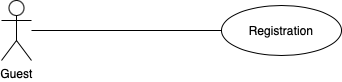
\includegraphics[width=0.6\linewidth]{Images/UCD_Registration.png}
        \caption{Guest Diagram}
        \label{fig:class_diagram}%
    \end{center}
\end{figure}

\subsection{Student}
\begin{figure}[H]
    \begin{center}
        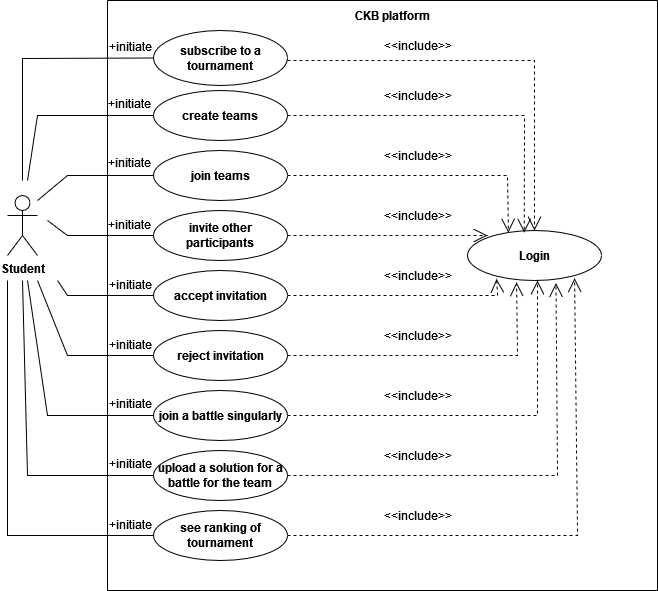
\includegraphics[width=0.8\linewidth]{Images/UCD_Student.png}
        \caption{Student Diagram}
        \label{fig:class_diagram}%
    \end{center}
\end{figure}
\subsection{Educator}
\begin{figure}[H]
    \begin{center}
        \includegraphics[width=0.8\linewidth]{Images/UCD_Educators.png}
        \caption{Educator Diagram}
        \label{fig:class_diagram}%
    \end{center}
\end{figure}

\section{Use Cases}
\label{subsec: use_case}%
\newcounter{uc}
\setcounter{uc}{1}
\newcommand{\cuc}{\theuc\stepcounter{uc}}
In this section, the primary identified use cases are elucidated. 
Each use case is accompanied by a table delineating entry conditions, event flow, exit conditions, and exceptions. 
Additionally, a sequence diagram is provided to illustrate the interactions between entities and the functions invoked. 
This comprehensive representation aims to capture the essential aspects of each use case, ensuring a clear understanding of the system dynamics within the context of the Code Kata Battle (CKB) platform.
\subsubsection*{UC\cuc . Student Registration}
\begin{center}
    \begin{longtable}{lp{0.75\linewidth}}
        \hline
        Actor            & Unregistered Student                                                                                                                                                                               \\
        \hline
        Entry conditions & The student isn't registered on the \verb|CKB| platform and clicks the sign-up button                                                                                                               \\
        \hline
        Event Flow       
        & 1. The \verb|CKB| platform prompts the unregistered student to input personal information (name, surname, email linked to an institutional profile).\\
        & 2. The unregistered student fills the form with personal information\\
        & 3. The student agrees to the platform's "Terms \& Conditions," and "Privacy Policy."\\
        & 4. The \verb|CKB| platform validates the provided student information.\\
        & 5. The \verb|CKB| platform requests the student to input a username for their profile.\\
        & 6. The student inputs a username.\\ 
        & 7. The \verb|CKB| platform validates the username.\\
        & 8. The \verb|CKB| platform sends a verification email containing a 6-digit code to the student's provided institutional email address.\\
        & 9. The \verb|CKB| platform prompts the student to input the verification code.\\
        & 10. The student inputs the verification code.\\
        & 11. The \verb|CKB| platform communicates the outcome of the student's registration.\\
        \hline
        Exit condition   & An account is created.   \\                                                                                                                                                                           
        \hline
        Exceptions   
        & 3.1. The student does not agree to the platform's "Terms \& Conditions," and "Privacy Policy."\\
            & The \verb|CKB| platform shows a message asking the user to agree to such "Terms \& Conditions" stopping the sign up operation.  \\                                                                                                   
        & 4.1. The \verb|CKB| platform is unable to validate the student's personal information.  \\                                                                                                         
            & In these cases, the unregistered student receives a notification with an error message.   \\
        & 7.1. The student's provided username is already in use.           \\                                                                                                
            & The \verb|CKB| platform shows a message asking the user to choose another username.   \\
        & 7.2. The student's provided username is in a non acceptable format    \\
            & The \verb|CKB| platform shows a message asking the user to choos another username    \\
      % email not received by user                                                                                        \\
        & 10.1. The student inputs an incorrect verification code.      \\                                                           
            & The \verb|CKB| platform shows a message asking the user to input the correct verification code.  \\
                                                                                        
        \hline
        \caption{Student Registration Use Case.}
        \label{tab: student_registration_use_case}
    \end{longtable}

    %QUI SEQUENCE DIAGRAM
    %\begin{comment}
    %    \begin{figure} [H]
    %        \begin{center}
                %\includegraphics[width=0.9\linewidth]{Images/SequenceDiagrams/student_registration}
   %             \caption{Student Registration Sequence Diagram}
%                \label{fig: student_registration_seq_diag}
    %        \end{center}
   %     \end{figure}
    %    \end{comment}
\end{center}

\subsubsection*{UC\cuc . User Login}
\begin{center}
    \begin{longtable}{lp{0.75\linewidth}}
        \hline
        Actor            & Registered User                                                                                                                                                                               \\
        \hline
        Entry conditions & The User is registered on the \verb|CKB| platform and clicks the login button.                                                                                                               \\
        \hline
        Event Flow       
        & 1. The \verb|CKB| platform prompts the user to input institutional email.\\
        & 2. The \verb|CKB| platform validates the email redirecting the user to the institution's page.\\
        & 3. The \verb|CKB| platform communicates the outcome of the user's login.\\
        \hline
        Exit condition   & Login completed.   \\                                                                                                                                                                           
        \hline
        Exceptions   
        & 2.1. The user's email isn't valid.\\                                          
        & 2.2. The user's verification on the institution's page goes wrong. \\                                                                                                         
            & In these cases, the user receives a notification with an error message.   \\                                                               
        \hline
        \caption{User Login Use Case.}
        \label{tab: user_login_use_case}
    \end{longtable}

    %QUI SEQUENCE DIAGRAM
    %\begin{comment}
    %    \begin{figure} [H]
    %        \begin{center}
                %\includegraphics[width=0.9\linewidth]{Images/SequenceDiagrams/student_registration}
   %             \caption{Student Registration Sequence Diagram}
%                \label{fig: student_registration_seq_diag}
    %        \end{center}
   %     \end{figure}
    %    \end{comment}
\end{center}

\subsubsection*{UC\cuc . Student Subscription to a Tournament}
\begin{center}
    \begin{longtable}{lp{0.75\linewidth}}
        \hline
        Actor            & Registered Student                                                                                                                                                                               \\
        \hline
        Entry conditions & The Student is logged in on the \verb|CKB| platform and clicks to the subscription button to a tournament.                                                                                                            \\
        \hline
        Event Flow       
        & 1. The \verb|CKB| platform receives the request.\\
        & 2. The \verb|CKB| platform checks if the tournament's subscription deadline is over.\\
        & 3. The \verb|CKB| platform communicates the outcome of the student's subscription.\\
        \hline
        Exit condition   & Subscription completed.   \\                                                                                                                                                                           
        \hline
        Exceptions   
        & 2.1. The tournament's subscription deadline is over.\\                                                                                                                                              
            & In these cases, the student receives a notification with an error message.   \\                                                               
        \hline
        \caption{Student Subscription Use Case.}
        \label{tab: student_subscription_use_case}
    \end{longtable}

    %QUI SEQUENCE DIAGRAM
    %\begin{comment}
    %    \begin{figure} [H]
    %        \begin{center}
                %\includegraphics[width=0.9\linewidth]{Images/SequenceDiagrams/student_registration}
   %             \caption{Student Registration Sequence Diagram}
%                \label{fig: student_registration_seq_diag}
    %        \end{center}
   %     \end{figure}
    %    \end{comment}
\end{center}
\subsubsection*{UC\cuc . Educator creates a tournament}

\begin{center}
    \begin{longtable}{lp{0.75\linewidth}}
        \hline
        Actor            & Unregistered Student                                                                                                                                                                               \\
        \hline
        Entry conditions & The educator is logged in on the \verb|CKB| platform.\\                                                                                                               \\
        \hline
        Event Flow       
        & 1. The educator clicks on the "Create Tournament" button from the Menu in the homepage.\\
        & 2. The \verb|CKB| platform prompts the educator to input the tournament name.\\
        & 3. The educator inputs the tournament name.\\
        & 4. The \verb|CKB| platform prompts the educator to input the registration deadline.\\
        & 5. The educator inputs the registration deadline.\\
        & 6. The educator toggles the "Advanced Options" section.\\
        & 7. The \verb|CKB| platform prompts the educator to choose whether to include badges or not.\\
        & 8. The educator chooses whether to include badges or not.\\
        & 9. The \verb|CKB| platform prompts the educator to choose which badges to include.\\
        & 10. The educator chooses which badges to include.\\
        & 11. The \verb|CKB| platform prompts the educator to choose whether to create new badges or not.\\
        & 12. The educator chooses to create new badges.\\
        & 13. The \verb|CKB| platform opens a pop-up window allowing the educator to create new badges by selecting and combining variables and rules.\\
        & 14. The educator creates new badges.\\
        & 15. The educator pushes the "Create Tournament" button.\\
        & 16. The \verb|CKB| platform communicates the outcome of the tournament creation.\\
        & 17. The \verb|CKB| platform notifies all students that a new tournament is available.\\
        \hline
        Exit condition   & A tournament is created.   \\                                                                                                                                                                         
        \hline
        Exceptions   
        & 3.1. The educator does not input the tournament name.\\
            & The \verb|CKB| platform shows a message asking the user to input the tournament name.  \\
        & 5.1. The educator does not input the registration deadline or inputs an invalid date.\\
            & The \verb|CKB| platform shows a message asking the user to input the registration deadline.  \\
        & 8.1. The educator does not choose whether to include badges or not.\\
            & The \verb|CKB| platform assumes that badges are not included.  \\
        & 10.1. The educator does not choose which badges to include.\\
            & The \verb|CKB| platform assumes that no pre-existing badges are included.  \\
        & 12.1. The educator does not choose to create new badges.\\
            & The \verb|CKB| platform assumes that no new badges are created.  \\
        & 14.1. The educator tries to create a new badge without selecting any variable or rule.\\
            & The \verb|CKB| platform shows a message asking the user to select at least one variable or rule.  \\
        \hline
        \caption{Tournament Creation Use Case.}
        \label{tab: tournament_creation_use_case}
    \end{longtable}

    %QUI SEQUENCE DIAGRAM
    %\begin{comment}
    %    \begin{figure} [H]
    %        \begin{center}
                %\includegraphics[width=0.9\linewidth]{Images/SequenceDiagrams/tournament_creation}
   %             \caption{Tournament Creation Sequence Diagram}
%                \label{fig: tournament creation_seq_diag}
    %        \end{center}
   %     \end{figure}
    %    \end{comment}
\end{center}


\section{Performance Requirements}
\label{subsec:performance_requirements}%

\subsection*{1. Response Time:}
   - The \verb|CKB| platform shall respond to user interactions within an average time of 2 seconds, measured from the user action initiation to the completion of the corresponding operation.

\subsection*{2. Concurrent Users:}
   - The platform should support at least 1000 concurrent users without a significant degradation in response time.

\subsection*{3. GitHub Integration:}
   - GitHub repository creation and updates triggered by student commits shall be processed within 5 minutes of the GitHub action.

\subsection*{4. Automated Evaluation:}
   - Automated evaluation of submitted code shall be completed within 1 minute of each GitHub push action.

\subsection*{5. Scalability:}
   - The platform should accommodate at least a 20\% annual increase in user base and battle participation.

\subsection*{6. Data Retrieval Time:}
   - Information retrieval for ongoing tournaments, tournament ranks, and personal scores should be performed within an average time of 3 seconds.

\subsection*{7. Consolidation Stage:}
   - The consolidation stage, where manual evaluation is required, should be completed within 3 days after the submission deadline of a battle.

\subsection*{8. Badge Assignment:}
   - Badge assignment based on rules and variables should be executed within 1 day after the final tournament rank becomes available.

\subsection*{9. Platform Uptime:}
   - The platform should maintain a minimum of 99.9\% uptime over any given month.

\subsection*{10. Notification Latency:}
    - Notifications should be sent to all relevant users within 1 minute of the triggering event.

\subsection*{11. Gamification Features:}
    - Display of badges on user profiles and visualization of tournament-related achievements should be accessible within a response time of 3 seconds.

\subsection*{12. API Response Time:}
    - External APIs used for integrations should respond within 5 seconds.

\subsection*{13. Load Testing:}
    - The platform should undergo periodic load testing to handle peak loads without compromising performance.

\subsection*{14. Security Scan Duration:}
    - Security scans during code quality evaluation should not exceed 2 minutes.







\begin{comment}
\section{Performance Requirements}
\label{subsec:performance_requirements}%

\subsection*{1. Response Time:}
   - The CKB platform shall respond to user interactions (e.g., creating a battle, joining a battle, submitting code) within an average time of 2 seconds, measured from the user action initiation to the completion of the corresponding operation.

\subsection*{2. Concurrent Users:}
   - The platform should support at least 1000 concurrent users participating in different battles and tournaments without a significant degradation in response time.

\subsection*{3. GitHub Integration:}
   - GitHub repository creation and updates triggered by student commits shall be processed and reflected in the CKB platform within 5 minutes of the GitHub action.

\subsection*{4. Automated Evaluation:}
   - The automated evaluation of submitted code, including functional aspects, timeliness, and quality level, shall be completed within 1 minute of each GitHub push action.

\subsection*{5. Scalability:}
   - The CKB platform should be designed to handle a growth in the number of users, battles, and tournaments. It should accommodate at least a 20\% annual increase in user base and battle participation.

\subsection*{6. Data Retrieval Time:}
   - Information retrieval for ongoing tournaments, tournament ranks, and personal scores should be performed within an average time of 3 seconds.

\subsection*{7. Consolidation Stage:}
   - The consolidation stage, where manual evaluation is required, should be completed within 3 days after the submission deadline of a battle.

\subsection*{8. Badge Assignment:}
   - Badge assignment based on rules and variables should be executed within 1 day after the final tournament rank becomes available.

\subsection*{9. Platform Uptime:}
   - The CKB platform should maintain a minimum of 99.9\% uptime over any given month to ensure continuous availability for users.

\subsection*{10. Notification Latency:}
    - Notifications, such as battle creation, submission deadlines, and tournament closure, should be sent to all relevant users within 1 minute of the triggering event.

\subsection*{11. Gamification Features:}
    - The display of badges on user profiles and the visualization of tournament-related achievements should be accessible with a response time of 3 seconds.

\subsection*{12. API Response Time:}
    - Any external APIs used for integrations, such as GitHub Actions and static analysis tools, should respond within 5 seconds to avoid delays in platform functionalities.

\subsection*{13. Load Testing:}
    - The platform should undergo periodic load testing to ensure it can handle peak loads and unexpected spikes in user activity without compromising performance.

\subsection*{14. Security Scan Duration:}
    - The time required for security scans during the evaluation of code quality should not exceed 2 minutes.

\end{comment}


\section{Design Constraints}
\label{sec:design_constraints}%

\subsection{Standards Compliance}
\label{subsec:standards_compliance}%
The Code Kata Battle (CKB) platform must conform to established standards and legal requirements to ensure ethical and lawful operation. Key considerations include:

\begin{enumerate}
    \item \textbf{Privacy and Data Laws:}
          \begin{itemize}
              \item The platform must adhere to all laws governing privacy and data treatment, especially regarding user information and data exchange with third parties, such as CodeKata educators.
              \item Compliance with the European Union General Data Protection Regulation (EU GDPR) is mandatory to ensure the privacy and rights of users are protected.
          \end{itemize}

    \item \textbf{EU GDPR Principles:}
          \begin{itemize}
              \item The system design should align with the principles outlined in Article 5 of the GDPR document, emphasizing the lawful, fair, and transparent processing of personal data.
          \end{itemize}
\end{enumerate}

\subsection{Hardware Limitations}
\label{subsec:hardware_limitations}%
The design and functionality of the CKB platform need to consider specific limitations for optimal user experience:

\begin{enumerate}
    \item \textbf{Cross-Platform Accessibility:}
          \begin{itemize}
              \item The platform should be accessible from both web browsers and mobile applications. Mobile applications will be implemented for Android and iOS operating systems.
          \end{itemize}
\end{enumerate}
\textbf{Note:} Cross-platform accessibility, although listed under hardware limitations, primarily involves software compatibility rather than hardware constraints. It highlights the need for the platform to function seamlessly across different operating systems.

\subsection{Other Constraints}
While considering standard compliance and hardware limitations, additional constraints specific to the CKB project should be acknowledged:

\begin{enumerate}
    \item \textbf{Educator Configuration:}
          \begin{itemize}
              \item The design should facilitate easy configuration by educators, allowing them to customize scoring criteria, badge rules, and associated variables according to their preferences and requirements.
          \end{itemize}

    \item \textbf{Automated Testing Tools:}
          \begin{itemize}
              \item Seamless integration with automated testing tools is essential. The platform should be designed to accommodate any constraints or limitations imposed by these tools during code evaluation.
          \end{itemize}

    \item \textbf{Scalability:}
          \begin{itemize}
              \item The platform must be scalable to handle a growing user base, increasing numbers of battles, and additional features without compromising performance. Consideration should be given to both the user interface and backend infrastructure.
          \end{itemize}

    \item \textbf{Educator Workload:}
          \begin{itemize}
              \item The design should optimize the educator's workload, particularly during the manual evaluation stage. Streamlining the evaluation process will enhance efficiency and user satisfaction.
          \end{itemize}

    \item \textbf{Gamification Logic:}
          \begin{itemize}
              \item Constraints associated with the gamification logic, including badge creation, rule definition, and variable association, should be carefully considered to maintain system flexibility without compromising integrity.
          \end{itemize}

    \item \textbf{Integration with External Systems:}
          \begin{itemize}
              \item The platform needs to seamlessly integrate with external systems, such as GitHub, while considering any constraints or limitations imposed by these external systems on data exchange and interactions.
          \end{itemize}
\end{enumerate}

These design constraints are vital to guide the development of the Code Kata Battle platform, ensuring legal compliance, optimal user experience, and consideration of specific project-related constraints.




\section{Software System Attributes}
\label{sec:software_system_attributes}%

\subsection{Reliability}
\label{subsec:reliability}%
The reliability of the Code Kata Battle (CKB) platform is crucial for its users, especially during critical operations such as code evaluations and scoring. 
While the platform doesn't require absolute perfection in every operation, it must maintain a high level of reliability to instill confidence in educators and students. 
Considering the nature of the platform, a failure rate between $0.1\%$ and $1\%$ is deemed acceptable. 
This range positions the CKB system as a robust and dependable tool for code kata battles.

\subsection{Availability}
\label{subsec:availability}%
Availability is a key attribute for the CKB platform, particularly for educators who rely on its functionalities for managing tournaments, battles, and student assessments. 
Downtime, especially during crucial periods like ongoing battles or tournament deadlines, is unacceptable. Therefore, the platform aims to achieve a remarkable $99.9\%$ uptime, ensuring educators have uninterrupted access to critical features. 
This commitment to high availability enhances the overall user experience and reinforces the platform's reliability.

\subsection{Security}
\label{subsec:security}%
Security is paramount for the CKB platform, given its involvement in handling code submissions, communication with external systems like GitHub, and the storage of sensitive user information. 
The platform ensures data privacy by employing HTTPS for secure communication. Additionally, all stored information is encrypted, providing an extra layer of protection against potential security threats. 
By prioritizing these security measures, the CKB platform safeguards the integrity and confidentiality of user data, fostering trust among educators and students.

\subsection{Maintainability}
\label{subsec:maintainability}%
Maintainability is a critical aspect of the CKB platform's design philosophy. The platform is structured into modular components to facilitate efficient maintenance, updates, and future extensions. 
Each implemented functionality is meticulously documented, ensuring clarity for developers involved in maintenance tasks. 
The design emphasizes a modular approach, allowing updates to specific components without adversely affecting the entire system. 
This commitment to maintainability ensures that the CKB platform can adapt to evolving requirements and technologies without compromising its stability.

\subsection{Portability}
\label{subsec:portability}%
The CKB platform prioritizes portability to accommodate a diverse user base. Users can access the platform seamlessly from web browsers and mobile applications on both Android and iOS devices. 
The choice of programming languages and development tools is a strategic decision, with the goal of providing a consistent user experience across different platforms. 
While cross-platform development tools offer efficiency, separate implementations for Android and iOS are considered for a more tailored user experience. 
This flexibility in portability ensures that the CKB platform remains accessible and user-friendly, regardless of the chosen device or operating system.
